\documentclass{article}

\usepackage[spanish]{babel}
\usepackage[utf8]{inputenc}
\usepackage[T1]{fontenc}
\usepackage{graphicx}
\usepackage{hyperref}
\usepackage{courier}
\usepackage{listings}
\usepackage{xcolor}
\usepackage{blindtext}
\usepackage{scrextend}
\usepackage[document]{ragged2e}
\usepackage{multicol}
\usepackage{pgfgantt}
\usepackage{mathtools}
\usepackage{minted}
\usepackage{tikz}
\usepackage{longtable}
\usepackage{algorithm}
\usepackage[noend]{algpseudocode}
\usepackage{amsmath}
\usepackage{wrapfig,lipsum,booktabs}
\usepackage{fontspec}
 % % % % % % % %

\setmainfont{Calibri}

\hypersetup{
	colorlinks,
	linkcolor={blue!60!black},
	citecolor={blue!50!black},
	urlcolor={blue!80!black}
}

\usetikzlibrary{positioning,fit,calc}

\usemintedstyle{pastie}

\usepackage{array}
\newcolumntype{L}[1]{>{\raggedright\let\newline\\\arraybackslash\hspace{0pt}}m{#1}}
\newcolumntype{C}[1]{>{\centering\let\newline\\\arraybackslash\hspace{0pt}}m{#1}}
\newcolumntype{R}[1]{>{\raggedleft\let\newline\\\arraybackslash\hspace{0pt}}m{#1}}

\def\labelitemi{\textbf{--}}

\usepackage{anysize}
\marginsize{2.54cm}{2.54cm}{2.54cm}{2.54cm}

\usepackage{setspace}
%\onehalfspacing
\doublespacing

\makeatletter
\newcommand*{\MoveFitHeight}[1]{%
	\pgfmathsetlengthmacro\fit@inner@sep{%
		\pgfkeysvalueof{/pgf/inner xsep}%
	}%
	\pgfmathsetlengthmacro\fit@text@height{%
		\tikz@text@height
	}%
	\kern-\fit@inner@sep\relax
	\raisebox{\fit@text@height}[0pt][0pt]{#1}%
}
\makeatother

\newcommand{\bigO}[1]{$O({#1})$}

\setlength{\columnsep}{1cm}

%En caso de que LaTeX separe las palabras con - de manera incorrecta, usar
%\hyphenation{deci-sión,e-xa-men, otras palabras....}


\begin{document}
%--% Portada %------------------------------------------%
\centerline{Universidad de Carabobo}
\centerline{Facultad de Ciencia y Tecnologia}
\centerline{Sistemas Operativos}
\vspace{7cm}
\begin{centering}
	\hrule 	\vspace{0.4cm}
	{ \Huge \bfseries Gestión de Memoria \\[0.4cm] }
	\hrule \vfill
\end{centering}
\vfill
\centerline{Victor Tortolero, 24.569.609}
\centerline{\today}
\newpage
%-------------------------------------------------------%


%--% Cuerpo %-------------------------------------------%
\section*{Reubicación de memoria}
La reubicación es el proceso de vinculación de direcciones lógicas de cada proceso con direcciones físicas concretas.
Permite crear un espacio lógico independiente para cada proceso y el sistema.
Este proceso generalmente lo realiza el enlazador en conjunto con el symbol resolution, que se encarta de de buscar los archivos
y librerías y remplaza sus referencias simbólicas con direcciones de memoria usables antes de ejecutar el programa.

\begin{itemize}
	\item \textbf{Reubicación estática}: El proceso de transformación ocurre antes de que comience la ejecución del programa. Las direcciones lógicas son iguales a las físicas. Su meta
	es permitir la compartición transparente. El espacio de direcciones se debe reservar de manera contigua, y una vez reservado
	no puede moverse. No garantiza la protección entre procesos.
	
	\item \textbf{Reubicación dinámica}: El proceso de transformación ocurre en la ejecución del programa. Las direcciones lógicas son distintas a las físicas. Requiere un hardware especializado, la unidad de manejo de memoria (MMU). Su meta es tener protección entre procesos. El espacio de direcciones un proceso puede crecer o ser movido.
\end{itemize}
%-------------------------------------------------------%

\section*{Memory Management Unit (MMU)}
Es un hardware que traduce las direcciones virtuales a direcciones fisicas. Todas las referencias a memoria pasan por la MMU. La TLB
actua como cacha para la tabla de direcciones virtuales de la MMU.
Es responsable de todos los aspectos del manejo de memoria.
Este suma el registro de reubicacion base a la direccion virtual para obtener la direccion fisica, compara las direcciones con un registro limite.

\vspace{0.4cm}

\begin{figure}[h]
	\centering
	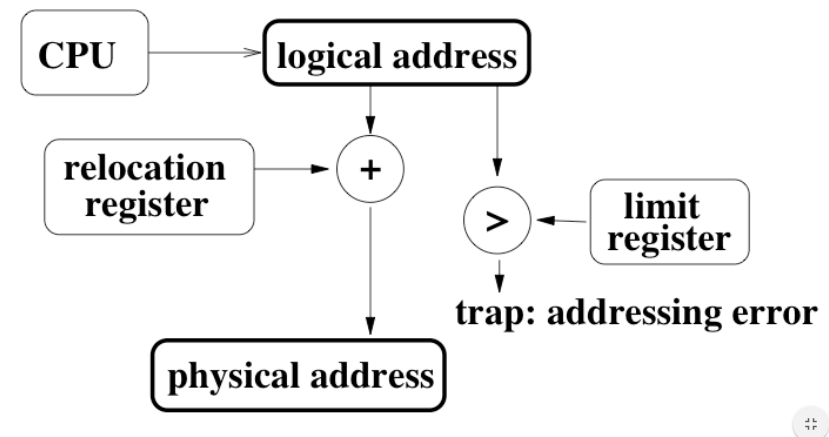
\includegraphics[scale=0.4]{img/mmu.png}
	\caption{Memory Management Unit}
\end{figure}

%--% Bibliografia %-------%
\newpage
\nocite{*}
\bibliographystyle{unsrt}
\bibliography{bibliography}
%--------------------------%
\end{document}
